\documentclass[11pt]{article}
\usepackage[a4paper,margin=2.2cm]{geometry}
\usepackage{booktabs}
\usepackage{graphicx}
\usepackage{array}
\usepackage[hidelinks]{hyperref}
\usepackage{caption}
\setlength{\parskip}{0.45em}
\setlength{\parindent}{0pt}
\graphicspath{{./}}

\title{Supplementary Material: Independent COMSOL Long-Window Follow-Up Experiment}
\author{}
\date{}

\begin{document}
\maketitle

\section*{Purpose and Scope}

This supplementary note reports an independent COMSOL follow-up experiment performed in response to the editor's concern that the original public-benchmark setting used a five-second observation window followed by a two-second extrapolation window. The purpose is to examine whether the proposed MI-PINN framework still mitigates error growth when the observation-free interval is extended.

The experiment is deliberately reported as an \emph{independent COMSOL follow-up}, not as a strict extension of the public Dou et al. benchmark data. The original manuscript results over the public benchmark remain defined by the selected 0--5 s observation window and 5--7 s extrapolation window. The present supplementary experiment uses newly generated COMSOL reference sequences and therefore should not be merged numerically with the public-benchmark RMSE or $R^2$ values.

\section*{Data and Sampling Protocol}

Two independent COMSOL 6.3 cases were used: a single-cylinder wake at $Re=100$ and a three-cylinder wake at $Re=100$. For both cases, the available time interval was 60--75 s with an output interval of $\Delta t=0.05$ s. The 60--65 s segment was used as the observation window, and 65--67 s, 65--70 s, and 65--75 s were used as progressively longer observation-free evaluation windows.

The spatial regions were matched to the selected learning windows used in the manuscript:
\begin{itemize}
\item Single-cylinder case: $[1,9]\times[-2,2]$.
\item Three-cylinder case: $[6,14]\times[-2,2]$.
\end{itemize}

The exported COMSOL fields were regridded to a spacing of $\Delta x=\Delta y=0.05$, giving $161\times81=13041$ spatial points for each case. Sparse observations were generated from $N_a=2000$ fixed Eulerian virtual probes selected within the corresponding region. Velocity labels were used only in the observation window. During the extrapolation window, velocity observations were masked; the models were evaluated against the reserved COMSOL reference fields after training.

\begin{table}[htbp]
\centering
\caption{Training and evaluation protocol for the independent COMSOL follow-up experiment.}
\small
\begin{tabular}{ll}
\toprule
Item & Setting \\
\midrule
Observation window & 60--65 s \\
Evaluation windows & 65--67 s, 65--70 s, 65--75 s \\
Output time step & $\Delta t=0.05$ s \\
Virtual probes & $N_a=2000$ fixed Eulerian probe locations \\
Observation mini-batch & $N_{\mathrm{obs}}=4000$ samples per iteration \\
Physics collocation mini-batch & $N_f=20000$ points per iteration \\
Mamba consistency mini-batch & $N_m=1140$ extrapolation-window samples \\
PINN optimization & 20000 Adam iterations \\
Mamba optimization in MI-PINN & 3000 Adam iterations \\
\bottomrule
\end{tabular}
\end{table}

Because this COMSOL follow-up uses $\Delta t=0.05$ s, a two-second direct prediction horizon corresponds to 40 time steps. This differs from the public benchmark setting in the manuscript, where $\Delta t=0.01$ s and a two-second horizon corresponds to 200 time steps. This difference is one reason why the follow-up experiment is reported separately from the main public-benchmark results.

\section*{Quantitative Results}

Table~\ref{tab:formal_results} reports speed-field $R^2$ and RMSE over the three progressively longer extrapolation windows. MI-PINN consistently reduces RMSE relative to the standard PINN baseline in both the single-cylinder and three-cylinder cases.

\begin{table}[htbp]
\centering
\caption{Independent COMSOL long-window follow-up results.}
\label{tab:formal_results}
\scriptsize
\begin{tabular}{llrrrrrr}
\toprule
Case & Method & $R^2$ 65--67 s & RMSE 65--67 s & $R^2$ 65--70 s & RMSE 65--70 s & $R^2$ 65--75 s & RMSE 65--75 s \\
\midrule
Single & PINN & 0.835830 & 0.097489 & 0.266361 & 0.205805 & -0.962353 & 0.335503 \\
Single & MI-PINN & 0.982278 & 0.032031 & 0.982181 & 0.032074 & 0.970701 & 0.040995 \\
Three & PINN & 0.775118 & 0.095083 & -1.000723 & 0.277456 & -2.783403 & 0.390878 \\
Three & MI-PINN & 0.902198 & 0.062704 & 0.822908 & 0.082547 & 0.734057 & 0.103632 \\
\bottomrule
\end{tabular}
\end{table}

\begin{table}[htbp]
\centering
\caption{RMSE reduction of MI-PINN relative to PINN in the independent COMSOL follow-up experiment.}
\small
\begin{tabular}{lrrr}
\toprule
Case & 65--67 s & 65--70 s & 65--75 s \\
\midrule
Single & 67.14\% & 84.42\% & 87.78\% \\
Three & 34.05\% & 70.25\% & 73.49\% \\
\bottomrule
\end{tabular}
\end{table}

\begin{figure}[htbp]
\centering
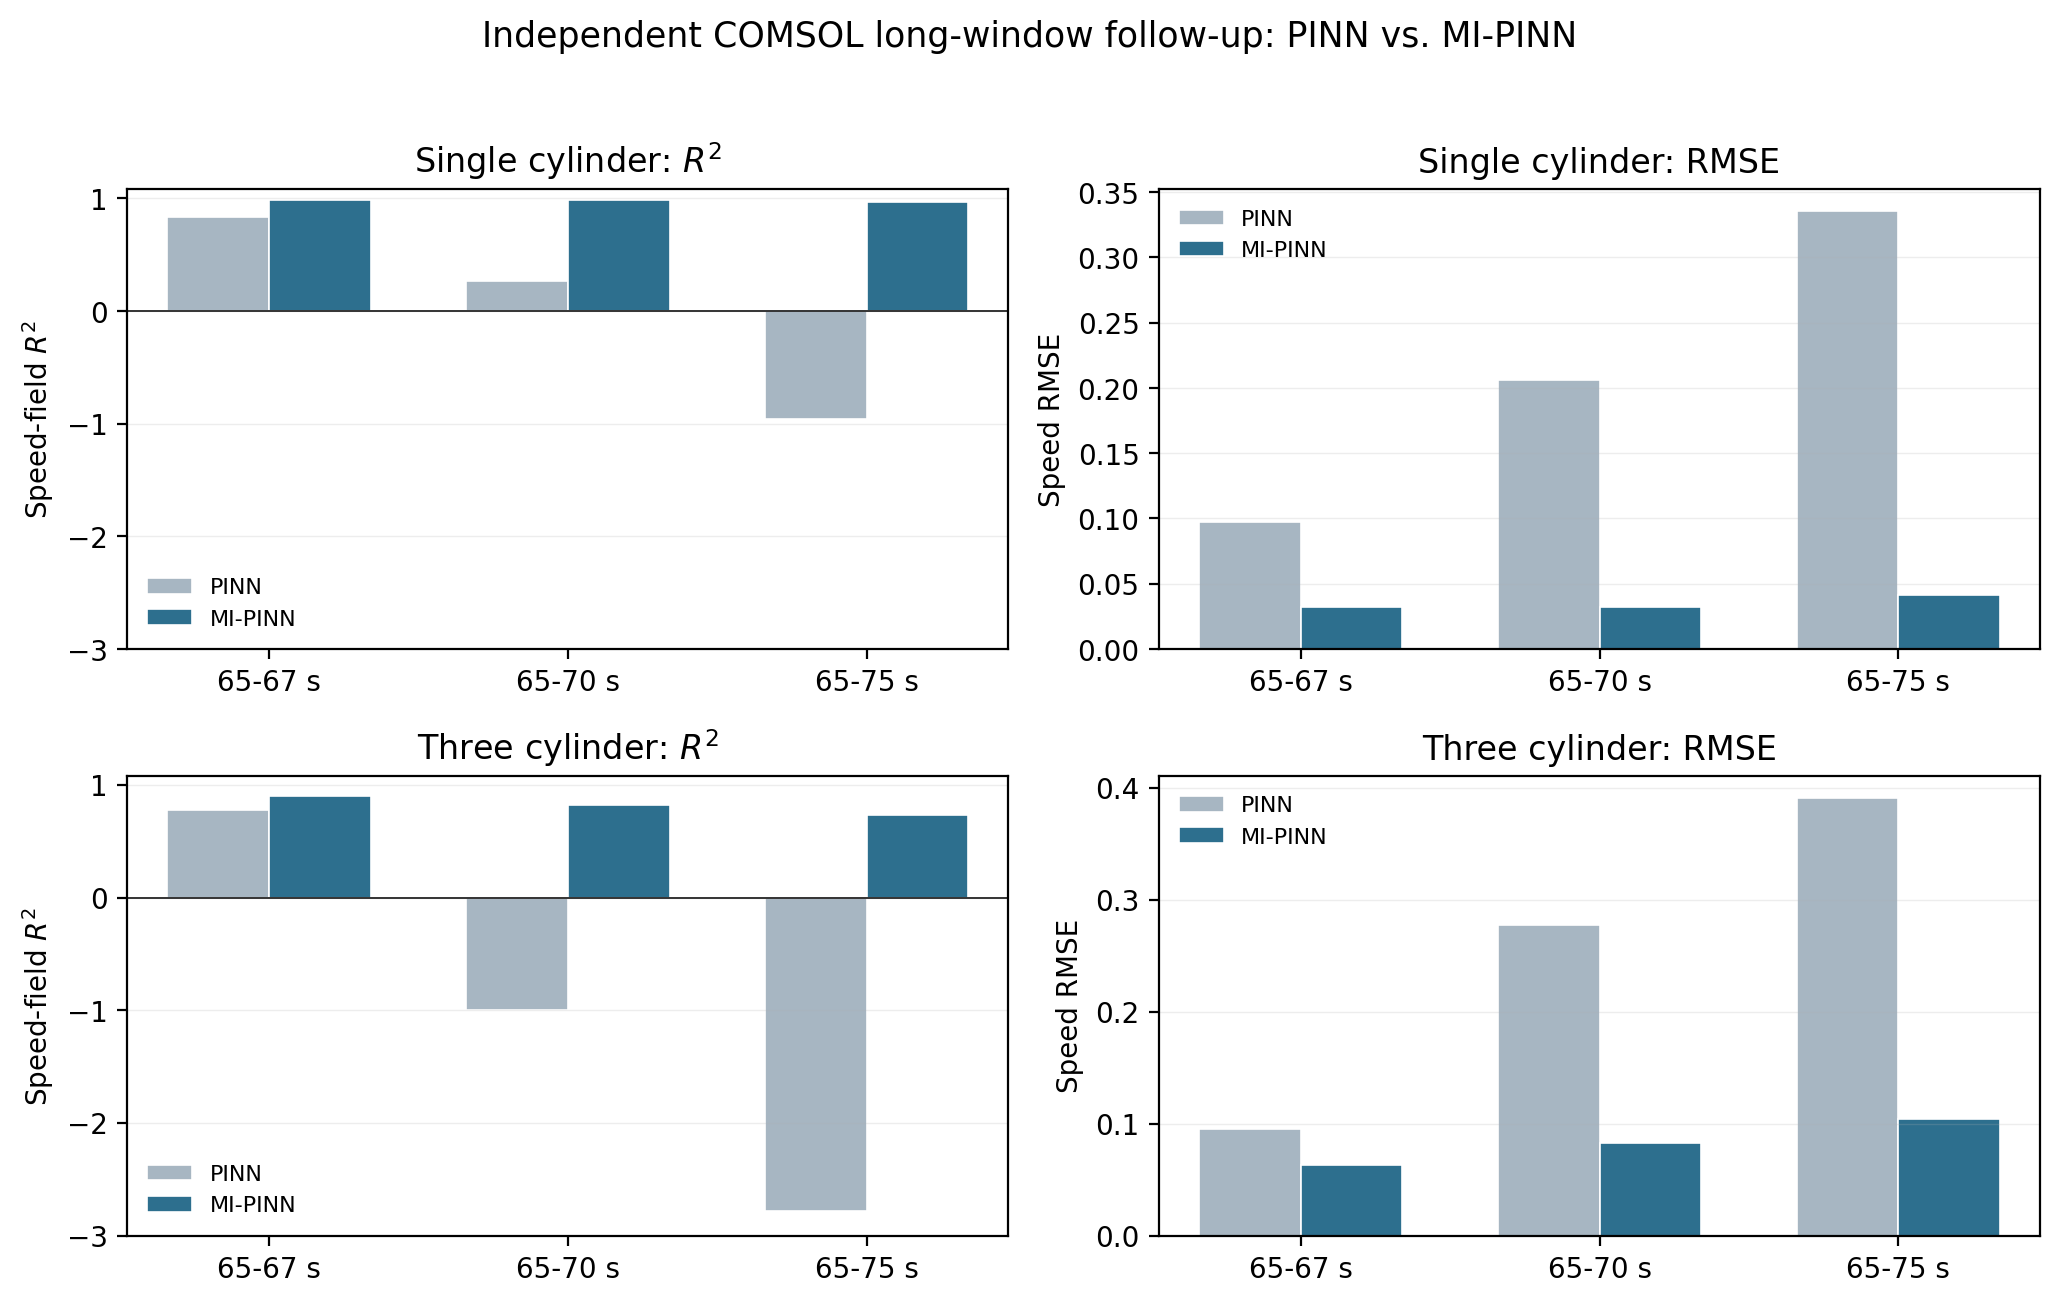
\includegraphics[width=0.96\textwidth]{editor2_formal_long_window_summary.png}
\caption{Independent COMSOL long-window follow-up experiment. The standard PINN baseline shows clear error growth as the observation-free interval is extended, whereas MI-PINN retains higher speed-field $R^2$ and lower RMSE in both cylinder-wake cases.}
\end{figure}

\section*{Interpretation}

The follow-up experiment supports a limited but useful conclusion. Under the independent COMSOL setting, the standard PINN baseline deteriorates substantially as the observation-free window is extended from 2 s to 5 s and 10 s. In contrast, MI-PINN maintains higher field-level accuracy, indicating that the Mamba-based temporal-prior consistency term helps reduce extrapolation error growth in the tested longer-window setting.

This evidence does not prove arbitrary long-term forecasting ability, nor does it convert the original public benchmark into a long-horizon benchmark. It instead provides an additional, traceable, independent-COMSOL result showing that the proposed temporal-prior mechanism remains beneficial when a longer reference sequence is available.

\section*{Traceability}

The corresponding formal-training run suffixes are:

\begin{center}
\small
\begin{tabular}{lll}
\toprule
Case & Method & Run suffix \\
\midrule
Single & PINN & \texttt{single/pinn/run\_20260611\_163150} \\
Single & MI-PINN & \texttt{single/mipinn/run\_20260611\_165753} \\
Three & PINN & \texttt{three/pinn/run\_20260611\_171830} \\
Three & MI-PINN & \texttt{three/mipinn/run\_20260611\_173245} \\
\bottomrule
\end{tabular}
\end{center}

\end{document}
